\documentclass[UTF8]{article}
\usepackage{pagecolor,lipsum}
\usepackage{amsmath}
\usepackage{amsfonts}
\usepackage{amssymb}
\usepackage{amsthm}
\usepackage{centernot}
\usepackage{tikz}
\usepackage{xcolor}
\usepackage{fullpage}
\usepackage[inline]{asymptote}
\usepackage{listings}
\usetikzlibrary{arrows,decorations.pathmorphing,backgrounds,positioning,fit,petri}
\newtheorem{theorem}{Theorem}
\newtheorem{defintion}{Definition}
\newtheorem{collorary}{Collorary}
\newtheorem{example}{Example}
\newtheorem{remark}{Remark}
\newtheorem{note}{Note} 
% no indentation
\setlength\parindent{0pt}

\begin{document}
Polish or prefix notation is expression can be evaluated without any parenthesis without any ambiguity
\begin{tikzpicture}[level distance=1.5cm,
level 1/.style={sibling distance=3cm},
level 2/.style={sibling distance=1.5cm}]
\node {-}
child {node {+}
child {node {1}}
child {node {2}}
}
child {node {-}
child {node {3}}
child {node {4}}
}; 
\end{tikzpicture} 
$-,+, 1, 2, -, 3, 4$

\begin{center}
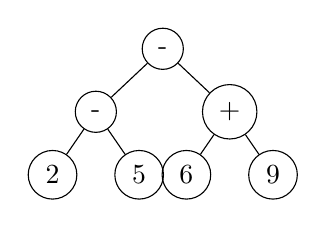
\begin{tikzpicture}[level distance=0.8cm,
level 1/.style={sibling distance=1.7cm},
level 2/.style={sibling distance=1.1cm}]
\tikzstyle{every node}=[circle,draw]
\node {-}
child {node {-}
child {node {2}}
child {node {5}}
}
child {node {+}
child {node {6}}
child {node {9}}
};
\end{tikzpicture}
\end{center} 

\end{document}
